\chapter{\IfLanguageName{dutch}{Stand van zaken}{State of the art}}%
\label{ch:stand-van-zaken}

% Tip: Begin elk hoofdstuk met een paragraaf inleiding die beschrijft hoe
% dit hoofdstuk past binnen het geheel van de bachelorproef. Geef in het
% bijzonder aan wat de link is met het vorige en volgende hoofdstuk.

% Pas na deze inleidende paragraaf komt de eerste sectiehoofding.

\begin{comment}

Dit hoofdstuk bevat je literatuurstudie. De inhoud gaat verder op de inleiding, maar zal het onderwerp van de bachelorproef *diepgaand* uitspitten. De bedoeling is dat de lezer na lezing van dit hoofdstuk helemaal op de hoogte is van de huidige stand van zaken (state-of-the-art) in het onderzoeksdomein. Iemand die niet vertrouwd is met het onderwerp, weet nu voldoende om de rest van het verhaal te kunnen volgen, zonder dat die er nog andere informatie moet over opzoeken \autocite{Pollefliet2011}.

Je verwijst bij elke bewering die je doet, vakterm die je introduceert, enz.\ naar je bronnen. In \LaTeX{} kan dat met het commando \texttt{$\backslash${textcite\{\}}} of \texttt{$\backslash${autocite\{\}}}. Als argument van het commando geef je de ``sleutel'' van een ``record'' in een bibliografische databank in het Bib\LaTeX{}-formaat (een tekstbestand). Als je expliciet naar de auteur verwijst in de zin, gebruik je \texttt{$\backslash${}textcite\{\}}.
Soms wil je de auteur niet expliciet vernoemen, dan gebruik je \texttt{$\backslash${}autocite\{\}}. In de volgende paragraaf een voorbeeld van elk.

\textcite{Knuth1998} schreef een van de standaardwerken over sorteer- en zoekalgoritmen. Experten zijn het erover eens dat cloud computing een interessante opportuniteit vormen, zowel voor gebruikers als voor dienstverleners op vlak van informatietechnologie~\autocite{Creeger2009}.

\end{comment}

% TODO ?


\section{Wat is Microsoft administration?}

In dit onderdeel wordt ...

% TODO Aanvulen

\subsection{Waarvoor staan Microsoft en administration?}

Microsoft administration bestaat uit twee kernwoorden die gekend zijn binnen de IT-wereld. Microsoft staat voor het Amerikaanse technologiebedrijf en de producten dat het aanbiedt \autocite{Warner2019}. Het woord administration, oftewel administratie in het Nederlands, staat voor het beheren van iets \autocite{Burgess2003}. Vanuit het woord administration volgde het woord administrator, dat duidt op een persoon die een of meerdere instanties beheerd. Microsoft administration staat voor het beheren van Microsoft-instanties en -producten waaronder Windows en Azure. 

% TODO Secundarie Bron zoeken voor Administrator ...

\subsection{Waarvoor staan Microsoft en administration?}

Het beheren van systemen kunnen omvat worden in een aantal taken, hieronder volgt een lijst van frequente taken tussen het jaar 1980 en 2000 \autocite{Frisch2002}.

\begin{itemize}
    \item Toevoegen van nieuwe gebruikers en toestellen
    \item Maken en beheren van back-ups
    \item Bestanden en andere data recupereren
    \item Gebruikers assisteren in dagelijkse taken en problemen
    \item Monitoren van systemen
    \item De veiligheid van de systemen garanderen
    \item Het beheren en installeren van updates
    \item Het automatiseren van taken
\end{itemize}

Deze taken zijn vandaag de dag nog steeds herkenbaar als dagdagelijkse taken van een systeembeheerder. 

\subsection{Wat houdt Microsoft administration in?}

Sinds de opkomst van Windows-systemen zoals Windows 2000 server, zijn er verschillende mogelijkheden om administratieve taken uit te voeren binnen netwerkinfrastructuren \autocite{Tulloch2001}. \\

Binnen Windows 2000 server zijn er administratieve tools zoals Microsoft Management Console, Event Viewer en Active Directory Domains and Trusts-instellingen beschikbaar. Deze tools dienen om de taken van een administrator te vergemakkelijken, door een overzicht te brengen van alle data in dat specifieke onderdeel \autocite{Sibisi2022}. Door het gebruik van deze administratieve tools kan een administrator Microsoft-entiteiten waaronder Windows-toestellen beheren om zijn taken mee uit te voeren. 

\subsection{Hoe evolueerde de systemen en de administratie hiervan doorheen de jaren?}

Rond het vroege begin van de $21^{ste}$ eeuw werden systemen en servers zoals Windows 2000 server met een focus op \ac{On-prem} onderhouden \autocite{Microsoft2022a}. \ac{On-prem} betekent dat software en hardware, zoals computers en servers, op locaties staan dat eigendom is van het bedrijf en lokaal worden toegepast \autocite{Gastermann2015}. Hierbij wordt de systeemadministratie door systeembeheerders lokaal aangepakt. Ter illustratie, in dit scenario wordt de automatisatie via PowerShell gefocust op de lokale entiteiten binnen het bedrijf. Databanken, mailservers, DNS-servers… worden lokaal aangesproken en geautomatiseerd indien nodig. \\

Rond het jaar 2006 evolueerde de On-premises-aanpak naar een cloud-aanpak \autocite{Hayes2008}. EC2 van Amazon is een van de grondleggers binnen de cloudservices \autocite{Qian2009}. Deze inventie van Amazon heeft sindsdien invloed op de huidige marktleiderspositie van AWS in cloud computing \autocite{Vailshery2022}. Op de tweede plaats bevindt zich de cloudservice van Microsoft, genaamd Azure. \\

\subsection{De impact van Cloud Computing}

Cloud Computing heeft een heel brede betekenis. Het is in feite een technologiemodel die wordt gebruikt om verschillende middelen en diensten beschikbaar te stellen op het internet, oftewel de cloud. \autocite{Haag2009} \\

De migratie van \ac{On-prem} naar de cloud is geen toeval. Eenenveertig procent van de bedrijven uit de \ac{EU} maakt gebruik van cloud computing in 2021. Het gebruik van cloud computing en cloudservices heeft vele voordelen. De volgende lijst bevat enkele voordelen van Cloud Computing. De lijst is samengesteld uit onderzoek van \textcite{Aljabre2012}, \textcite{Rittinghouse2016}.

\begin{itemize}
    \item Minder onderhouds-, implementatie en infrastructuurkosten
    \item Goedkopere computers per gebruiker (via virtuele machines)
    \item Verhoogde mobiliteitskansen voor de werkkrachten
    \item Nieuwe en flexibelere infrastructuren met meer schaalbaarheid
    \item Vergroening van data centers
    \item Verhoogde beschikbaarheid van applicaties
    \item Mogelijkheid om gebruikers te doen samenwerking in documenten en projecten
     
\end{itemize}

\subsection{Welke impact heeft de verschuiving van On-premises naar de cloud op Micosoft administration?}

De evolutie van \ac{On-prem} naar de cloud heeft invloed op de huidige stand van zaken binnen Microsoft administration. Microsoft administratie staat in voor het beheren van Microsoft-entiteiten. Door een verschuiving van \ac{On-prem} naar cloud-omgevingen, wordt de nadruk stilaan gelegd op het beheren van bepaalde entiteiten via cloud-toepassingen. \\

Deze nadruk valt op wanneer de productenlijst van Microsoft Azure wordt geraadpleegd \autocite{Microsoft2023b}. Dit is een lijst die steeds verder wordt uitgebreid met nieuwe technologieën. \\

Een praktisch voorbeeld van een entiteit, of een groep van entiteiten, dat via de cloud kan beheerd worden is Azure Active Directory \autocite{Microsoft2023c}. Azure Active Directory kan gebruikt worden als alternatief voor Active Directory voor bepaalde onderdelen. Active Directory is kortweg een opslagplaats die een focus heeft op On-premises-instanties. Active Directory en Azure Active Directory worden in het volgende onderdeel verder besproken.

% ---
% Volgende onderdeel
% ---

\section{Azure Active Directory Graph}

\subsection{Wat is Active Directory?}

\ac{AD} is een centrale en gemeenschappelijke opslagplaats voor informatie geïntroduceerd door Microsoft \autocite{Allen2003}. De eerste versie van \ac{AD} is gemaakt voor de Windows 2000 server-editie. Deze opslagplaats bevat allerlei informatie binnen een netwerk, zoals gebruikers, groepen, computers, applicaties, bestanden en printers. Deze informatie kan worden opgevraagd en beheerd.

\subsection{Wat is Azure Active Directory?}

Azure \ac{AD} is een modernere aanpak van Active Directory binnen de cloud dat ontstaan is in 2008 \autocite{Chappell2008}. Azure \ac{AD} is een gecentraliseerd beheerplatform van Microsoft voor gebruikers en apparaten in netwerken die een verbinding hebben met de Azure-clouddienst \autocite{Mayank2019}. Middelen, waaronder gebruikers en apparaten, kunnen vanuit Azure \ac{AD} beheerd worden met bijhorende netwerkauthenticatie. Het dient als een centraal punt van informatie, waarbij details over alle middelen in het netwerk worden opgeslagen.

\subsection{Wat is Azure Active Directory met PowerShell?} 

Azure \ac{AD} PowerShell voor Graph, kortweg Azure \ac{AD} PowerShell, is een module binnen PowerShell dat gebruikt kan worden om Azure \ac{AD} te beheren \autocite{Microsoft2023}. PowerShell is een oplossing van Microsoft voor taakautomatisering via een \ac{CLI} \autocite{Microsoft2022}. \\

PowerShell staat gekend voor zijn breed scala aan informatie dat het kan verkrijgen. Dit breed scala gaat van systemen, servers, randapparatuur, mobiele apparaten tot gegevensgestuurde toepassingen zoals Active Directory \autocite{Hosmer2019}. Vandaag de dag ondersteunt PowerShell meer dan 11.350 unieke modules en scripts via de PowerShell Gallary, waaronder de Azure \ac{AD} PowerShell module \autocite{Microsoft2023a}. \\

Door het gebruik van Azure \ac{AD} in combinatie met PowerShell, wordt er gebruikgemaakt van het beste van de twee werelden. Een gecentraliseerd beheerplatform automatisch doen werken brengt bijkomende voordelen voor de maker. Uit onderzoek van \textcite{Breton2003} zijn enkele voordelen van automatisatie minder stress, tijdbesparing en een lagere kans op menselijke fouten.

\subsection{Wat is Azure Active Directory Graph?}

De communicatie tussen Azure AD en de Azure AD PowerShell module gebeurd via een API. Deze API is een REST API dat Graph wordt genoemd. \\ 

De naam Graph is afgeleid uit het wiskundige figuur van een graaf. Een graaf is een verzameling van punten die wel of niet met elkaar zijn verbonden \autocite{Denaux2022}. Een voorbeeld van een wiskundige graaf is te zien op Figuur \ref{mga}. \\

\begin{figure}
    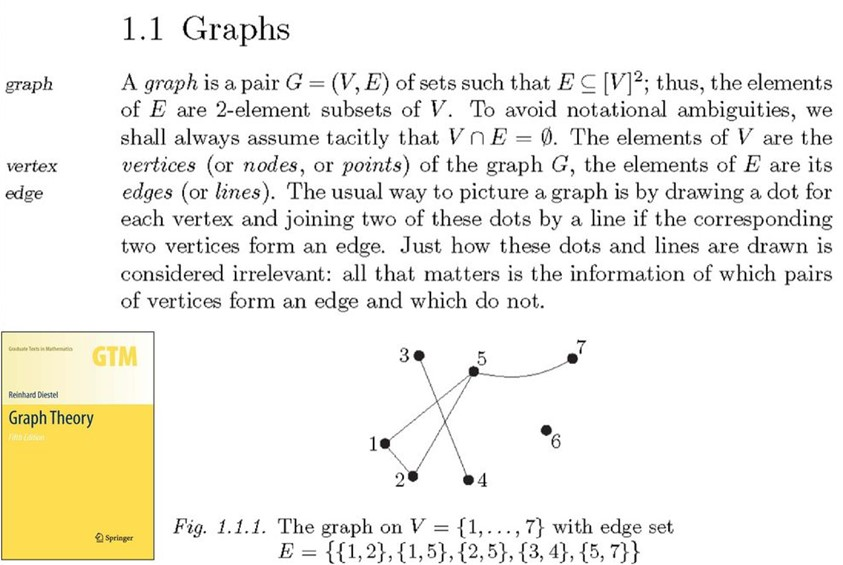
\includegraphics[width=\textwidth]{MathGraphExample.jpg}
    \caption[Voorbeeld wiskundige graaf]{Voorbeeld van een graaf in de wiskunde uit het boek Graph Theory van \textcite{Diestel2010}.}
    \label{mga}
\end{figure}

Graph van Microsoft heeft een soortgelijke betekenis als dat van een wiskundige graaf. Graph staat in voor de verbindingen tussen de entiteiten dat het ondersteunt, in dit geval Microsoft-entiteiten \autocite{Kokkarinen2022}. Een logische interpretatie van Graph wordt weergegeven op Figuur \ref{gms}.

\begin{figure}
    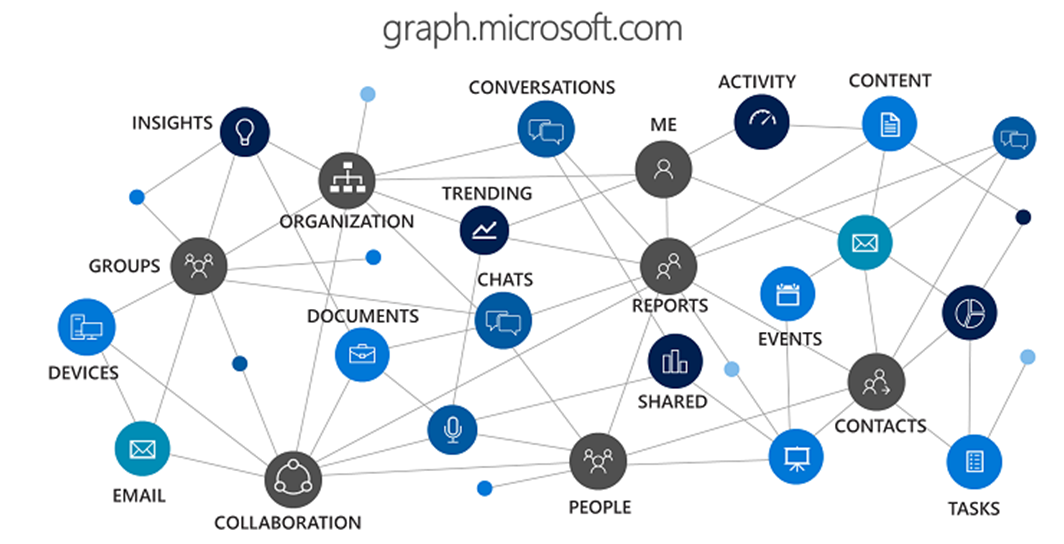
\includegraphics[width=\textwidth]{GraphMicrosoft.png}
    \caption[Voorbeeld Microsoft Graph]{Voorstelling van Graph door \textcite{Microsoft2017}.}
    \label{gms}
\end{figure}

\subsection{Toepassingen van Azure AD via PowerShell en Graph} 


\section{Microsoft Graph}

\lipsum[10-12]




